% 几何矢量
% 线性代数|几何矢量|代数矢量|单位矢量|标量|平行四边形法则|线性组合|线性相关|线性无关|基底|矢量空间|坐标

我们来回顾高中学的\textbf{几何矢量}, 本文中简称为“矢量”. 矢量是空间中的一些有长度有方向的箭头. 我们对它的位置不感兴趣, 所有长度和方向相同的矢量都视为同一矢量. 本书中矢量用正黑体表示, 如 $\bvec a$. 在手写时, 可以在字母上方加箭头表示, 如 $\overrightarrow{a}$. 特殊地, 如果一个矢量的长度等于 1, 那么它就是一个\textbf{单位矢量}, 本书中在矢量上面加上 “\^{}” 符号表示单位矢量, 如 $\uvec a$. 为了与矢量区分, 我们把单个的实数或复数称为\textbf{标量}.

从概念上来说几何矢量本身可以单独存在而不需要借助任何坐标系或坐标来描述. 例如在房梁上悬挂一支箭, 它有长度, 有方向, 就是一个矢量, 不需要任何参照物或者坐标系. 下面要介绍的许多概念(加法, 数乘, 线性组合, 线性无关等)都不需要任何坐标的概念, 请读者注意区分我们什么时候在讨论矢量本身什么时候在讨论它的坐标. 以后我们在学习矢量空间时会发现广义的矢量几乎可以是任何东西(多项式, 函数等等), 它们同样也可以具有坐标的概念(甚至可能是复数), 和我们下面要讨论的矢量也有许多相似的性质.

\subsection{矢量的加法}
如\autoref{GVec_fig1},两个矢量相加, 既可以使用平行四边形法则, 也可以用三角形法则. 若有多个矢量连续相加, 可以分别把它们首尾相接, 结果就是由起点指向终点的矢量. 容易证明矢量的加法满足加法交换律 $\bvec A + \bvec B = \bvec B + \bvec A$, 结合律 $(\bvec A + \bvec B) + \bvec C = \bvec A + (\bvec B + \bvec C)$.
\begin{figure}[ht]
\centering
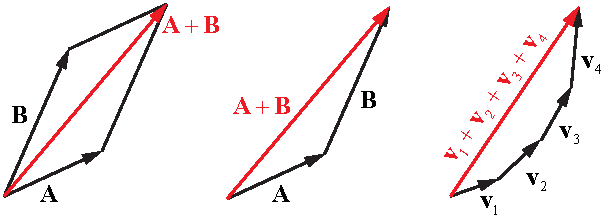
\includegraphics[width=10.5cm]{./figures/GVec_1.pdf}
\caption{矢量的加法} \label{GVec_fig1}
\end{figure}

\subsection{矢量的数乘\ 共线}
如\autoref{GVec_fig2}, 一个矢量与一个正实数相乘, 则方向不变, 把长度乘以这个实数. 若这个数是负数, 则把矢量取反方向再把长度乘以这个实数数的绝对值即可.若 $\lambda, \mu$ 表示实数, 容易证明分配律 $\lambda(\bvec A + \bvec B) = \lambda\bvec A + \lambda\bvec B$ 和 $(\lambda+\mu)\bvec A = \lambda\bvec A + \mu\bvec A$, 结合律 $\lambda(\mu\bvec A) = (\lambda\mu) \bvec A$.
\begin{figure}[ht]
\centering
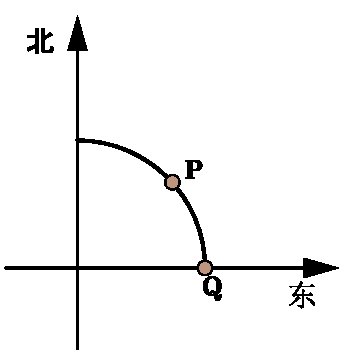
\includegraphics[width=6.5cm]{./figures/GVec_2.pdf}
\caption{矢量的数乘} \label{GVec_fig2}
\end{figure}

如果两个矢量的关系可以用 $\bvec A = \lambda\bvec B$ 表示, 那么它们就是\textbf{共线}的. 共线的充分必要条件\upref{SufCnd}是, 两矢量方向相同或相反.

\subsection{矢量的线性组合}
把若干矢量 $\bvec v_i$ 分别与若干实数 $c_i$ 相乘再相加就得到了这些矢量的一个\textbf{线性组合}
\begin{equation}\label{GVec_eq1}
\sum_i^N c_i \bvec v_i = c_1\bvec v_1 + c_2\bvec v_2 +\dots +c_N \bvec v_N
\end{equation}

\subsection{线性相关\ 线性无关}
如果存在至少一组不全为零系数 $c_i$ 使几个矢量的线性组合等于零, 这些矢量就被称为\textbf{线性相关}的
\begin{equation}\label{GVec_eq2}
\sum_i^N c_i \bvec v_i = \bvec 0
\end{equation}
这是因为对于任何一个不为零的项 $j$, 矢量 $\bvec v_j$ 都可以表示为其他矢量的线性组合. 只需把上式除以 $c_j$ 即可
\begin{equation}\label{GVec_eq3}
\bvec v_j = \sum_{i \ne j}\frac{c_i}{c_j} \bvec v_i
\end{equation}
如果不存在这样的系数, 这些矢量就是\textbf{线性无关}的. 

如果一组矢量之间线性相关,那么至少有一个矢量是“冗余”的,也就是说,它可以被其它矢量的线性组合表示出来.这样一来,对于线性相关的矢量组,如果用它们的线性组合来表示其它矢量,那么表示方式都不是唯一的.线性无关的矢量组,最重要的性质就是它们的线性组合表达式是唯一的,由此引入了基地、坐标等概念.

\subsection{基底\ 矢量空间\ 坐标}
沿一条直线的所有矢量都是共线的, 所以在一条直线上最多不超过一个矢量线性无关, 所有这些共线的矢量以及它们的加法和数乘运算组成一个\textbf{一维矢量空间}\footnote{注意这里并没不打算给出矢量空间的一般定义, 只是说 “是一个矢量空间”. 一般定义见 “矢量空间\upref{LSpace}”}. 一个平面上的所有矢量以及它们的加法和数乘运算, 组成一个\textbf{二维矢量空间}, 二维矢量空间中最多只能找到两个线性无关的矢量. \textbf{三维矢量空间}同理. 如无特殊说明, 我们只讨论不超过 3 维的几何矢量.

$N$ 维空间中的任意一组线性无关的 $N$ 个矢量 $\bvec \beta_1\dots \bvec \beta_N$ 可以作为一组\textbf{矢量基底}, 记为 $\{\bvec \beta_i\}$. 基底是有序的, 一旦确定就不能随意改变. 如果在这组基底中加入该空间中任意一个矢量 $\bvec v$, 这组 $N+1$ 个矢量必定线性相关(否则空间就是 $N+1$ 维的), 即存在不全为零的实数 $c_1\dots c_{N+1}$ 使下式成立
\begin{equation}
\sum_{i=1}^N c_i \bvec \beta_i + c_{N+1} \bvec v = \bvec 0
\end{equation}
我们还可以得知 $c_{N+1}$ 必不为零(反证法:如果 $c_{N+1} = 0$, 则可得出基底 $\{\bvec \beta_i\}$ 线性相关, 不成立), 所以由\autoref{GVec_eq3} 可知 $\bvec v$ 可用 $\{\bvec \beta_i\}$ 的线性组合表示. 令 $x_i = -c_i/c_{N+1}$, 该空间中任意矢量 $\bvec v$ 都有
\begin{equation}\label{GVec_eq5}
\bvec v = \sum_{i=1}^N x_i \bvec \beta_i
\end{equation}
这里的 $x_i$ 就是矢量空间中\textbf{坐标}的定义.

\begin{exercise}{计算坐标}
以上所说的坐标不一定是直角坐标系的坐标. 例如平面上两个基底 $\bvec \beta_1$ 与 $\bvec \beta_2$ 的长度分别为 1 和 2. 夹角为 $\pi/3$, 矢量 $\bvec v$ 恰好落在两个基底的角平分线上, 长度为 3. 求 $\bvec v$ 的坐标.答案:$1/\sqrt 3$, $1/(2\sqrt 3)$.
\end{exercise}

我们可以用反证法证明坐标的唯一性. 假设有两组不全相同的系数都可以使\autoref{GVec_eq5} 成立, 分别记为 $x_i$ 和 $y_i$. 那么分别代入上式再把两式相减得到
\begin{equation}
\sum_{i=1}^N (x_i-y_i) \bvec \beta_i = \bvec 0
\end{equation}
由于 $(x_i-y_i)$ 不全为零, 得到基底 $\{\bvec \beta_i\}$ 线性相关, 而这是不可能的.证毕.

\subsection{坐标的运算}
我们常常把一个矢量的坐标写成一个\textbf{代数矢量}, 如
\begin{equation}\label{GVec_eq7}
\bvec v = \pmat{x\\y\\z}_{\{\bvec\beta_i\}}
\end{equation}
在列矢量的右下角声明基底是较为严谨的做法, 但为了书写简洁, 在不至于混淆的情况下我们可以将其省略. 另外在正文中, 为了节约空间, 我们将\autoref{GVec_eq7} 记为 $\bvec v = (x, y, z)_{\{\bvec\beta_i\}}\Tr$(见“矩阵\upref{Mat}” \autoref{Mat_eq2} ), 同样, 我们时常省略 $\{\bvec\beta_i\}$.

当我们说两个矢量\textbf{相等}时, 同一基底下两矢量的坐标全都需要相等. 若已知两矢量在不同基底下的列矢量, 则需要先将它们变换到同一基底下再判断是否相等.

以上介绍的加法和数乘都有对应的坐标运算. 由\autoref{GVec_eq5} 及矢量加法和数乘的交换律和结合律得
\begin{equation}\label{GVec_eq8}
\bvec v_1 + \bvec v_2 = \pmat{x_1\\y_1\\z_1}_{\{\bvec\beta_i\}} + \pmat{x_2\\y_2\\z_2}_{\{\bvec\beta_i\}} = \pmat{x_1 + x_2\\y_1 + y_2\\z_1 + z_2}_{\{\bvec\beta_i\}}
\end{equation}
\begin{equation}\label{GVec_eq9}
\lambda \bvec v = \lambda\pmat{x\\y\\z}_{\{\bvec\beta_i\}} = \pmat{\lambda x\\\lambda y\\\lambda z}_{\{\bvec\beta_i\}}
\end{equation}

要特别注意的是, 当定义了多组基底时, 只有基底相同的两个列矢量按照\autoref{GVec_eq8} 相加才有意义.
